\documentclass[12pt]{article}

\usepackage{indentfirst}
\usepackage{hyperref}
\usepackage{graphicx}
\usepackage[margin=1in]{geometry}

\graphicspath{ {../data/003/visualisation_v2/} {../results/SLP/003/ROC/} }

\begin{document}
	\begin{center}

	    \vspace*{1cm}
	    \Large
	    Vilnius University

		Mathematics and Informatics Faculty

		Insitute of Informatics 

		Bioinformatics study program
	    
        \vspace*{4cm}
        \Large
		\textbf{Protein thermostability prediction using 
		sequence representations from protein 
		language models}

	\end{center}

	\begin{flushright}

		\vspace*{2cm}
        \large
        Author: Ieva Pudžiuvelytė

        Supervisor: Kliment Olechnovič, PhD 
        
	\end{flushright}

	\begin{center}
		\vspace*{4cm}
        \large
        Course thesis
        
        \vspace*{2cm}
        \large
        Vilnius, 2022
	\end{center}
	
	\newpage

	\tableofcontents

	\newpage
	
	\Large
	\section{Introduction}

    \vspace*{1cm}
        
	\normalsize

	The variety of proteins is no less diverse than the variety of organisms. 
	Just as the latter set is divided into domains, there are different 
	attempts to classify proteins into distinct subsets. One way is to 
	consider the heat-resistance property of biological macromolecules, which 
	is an important trait for practical applications, for example, PCR.

	Earlier studies show that protein's sequence and structural properties 
	influence the thermostability of the macromolecule \cite{modarres2016protein}. 
	Furthermore, one of the most recent achievements in the field of deep 
	learning are transformer architecture-based language models or, particularly, 
	protein language models that have not yet been used to classify proteins based on
	their thermostability. Therefore, it was decided to apply protein 
	representations from the protein language model to make inferences about 
	thermostability of the biological macromolecules.

	There are transformer architecture-based language models trained in an 
	unsupervised fashion to predict probabilities of elements in sequences 
	\cite{devlin2018bert}. 
	Simultaneously, the process of training creates sequences' embeddings – the 
	real numbered vectors that represent semantic connections of language 
	components. These representations can be transferred as input to specific 
	application models trained using a supervised learning method to complete 
	the defined task, such as the classification problem. Unsurprisingly, the 
	transition between two types of learning has a name of 'transfer learning'. 
	This separation is practically useful because the computationally-heavy 
	task to train the language model can be excluded from the development of 
	the application model.

	Since proteins can be represented in amino acid sequences assumed as a 
	particular language, there are protein language models – models trained on 
	protein sequences – that provide embeddings as output. The multi-dimensional 
	vectors are transferred for the application neural network as its input to 
	observe the results and decide whether the computed representations are 
	suitable to solve the specific biological task.

	This work presents a novel way to predict thermal stability of proteins. 
	The solution is a feed-forward neural network (FNN). To train the FNN, 
	the evolutionary scale model 1b (ESM-1b)\cite{rives2021biological} is used to 
	generate embeddings for proteins of organisms with annotated growth 
	temperatures \cite{engqvist_martin_karl_magnus_2018_1175609}. The model 
	takes the generated embedding to predict the thermostability class of the 
	input protein.

	\newpage

	\section{Theory}

	The main objective of the work is to apply embeddings from protein language 
	models to create a classifier that could determine to which thermostability 
	class the protein sequence belongs.

	Thermostability classes were created by setting the threshold of 
	$65\ ^\circ$C - proteins that are stable at temperatures strictly lower 
	than the given threshold should be assigned to class '0' and the 
	remaining ones compose the class '1'. 

	\subsection{Protein language models}

	Protein language models are transformer models trained on protein sequences.
	The transformer is a model, which is made of encoder-decoder architecture 
	that relies entirely on self-attention \cite{vaswani2017attention}. 
	The encoder part provides continuous representations of the input composed 
	of sequences of symbols, meanwhile the decoder part generates output for each 
	symbol in the input sequence. For this principle of architecture, transformers
	can be trained in an unsupervised fashion and be applies to natural language
	processing (NLP) tasks at which they produce state-of-the-art 
	results \cite{vig2019analyzing}.

	Since amino acid sequences can be considered as a particular language, 
	transformer architectures were applied to solve tasks related to protein 
	biology or molecule modeling \textit{in silico}. Attention mechanisms in 
	models of transformer architecture, taking BERT-like model as a example 
	\cite{vig2020bertology}, are capable to capture the folding structure, 
	binding sites, and complex biophysical properties of proteins.

	\subsection{ESM-1b embeddings}

	Due to the novelty of embeddings, a considerably good performance of
	protein language models, and a recently emerged availability of embeddings,
	it was decided to develop a neural network model that would take protein
	embeddings as input and give the thermostability class
	label as output.

	ESM-1b is one of evolutionary scale models trained by Facebook Research 
	\cite{rives2021biological}. The model has 33 layers and 650 million parameters. 
	The model was trained in an 
	unsupervised fashion on 
	\href{ftp://ftp.uniprot.org/pub/databases/uniprot/uniref/uniref50}{UniRef50 data set}
	(accessed March 28, 2018)\cite{suzek2015uniref}. In order 
	to ensure
	determinism in the validation set, authors removed protein sequences that
	were longer than 1024 amino acids. 

	The authors made a script to extract model's embeddings available in the 
	\href{https://github.com/facebookresearch/esm}{repository "Evolutionary Scale Modeling"}.
	The script allows to choose 
	from which model and layer embeddings will be taken, what embeddings 
	(mean, per amino acid, or beginning of the sequence token) to keep. In the
	result of using the script, a 1280 dimensional vector for each protein is 
	generated.
	
	The fact that sequences longer than 1024 amino acids were removed from the 
	validation data set for ESM-1b model's training implies to the limitation of 
	model's embeddings, which cannot be generated for sequences longer than 
	1024 amino acids.

	\newpage

	\section{Methods}

	Generally, the development of a tool for protein thermostability predictions
	consisted of the following steps:

	\begin{enumerate}
		\item Collecting sets of sequences
		\item Calculating ESM-1b embeddings for the sets of sequences
		\item Processing the set of generated embeddings
		\item Visualising ESM-1b embeddings
		\item Training and validating the neural network model of the chosen architecture 
		\item Testing the trained neural network model
		\item Presenting the results of the model
	\end{enumerate}

	The workflow will be reviewed in terms of these points.

	\subsection{Collecting data}

	Initially, the steps prior to the neural network model construction 
	were done using a small data set that was composed of proteomes of two 
	organisms: a mesophilic bacteria \textit{Escherichia coli} 
	(\href{https://www.uniprot.org/proteomes/UP000000625}{UP000000625}) and a 
	thermophilic archaeon \textit{Sulfolobus solfataricus} 
	(\href{https://www.uniprot.org/proteomes/UP000001974}{UP000001974}). The 
	growth temperature of \textit{E. coli} is $37\ ^\circ$C \cite{jang2017environmental}
	and $80\ ^\circ$C for \textit{S. solfataricus} \cite{zaparty2010hot}. This 
	data set was named '001' and used only for embeddings visualisation.

	The visualisation of '001' stimulated to check whether embeddings are 
	distinguished by the thermostability property or the life domain has a
	significant impact to the data clusterisation. Subsequently, '002' data set 
	was a collection of 2 mesophilic archaea and 2 thermophilic bacteria
	proteomes.

	\vspace*{0.5cm}

	Mesophilic archaea:

	\begin{itemize}
		\item \textit{Methanobrevibacter oralis} 
		(\href{https://www.uniprot.org/proteomes/UP000077428}{UP000077428})
		\item \textit{Nitrosopumilus maritimus} strain SCM1 (\href{https://www.uniprot.org/proteomes/UP000000792}{UP000000792})
	\end{itemize}

	Thermophilic bacteria:

	\begin{itemize}
		\item \textit{Aquifex aeolicus} (strain VF5)
		(\href{https://www.uniprot.org/proteomes/UP000000798}{UP000000798})
		\item \textit{Thermotoga maritima} 
		(strain ATCC 43589 / DSM 3109 / JCM 10099 / NBRC 100826 / MSB8) 
		(\href{https://www.uniprot.org/proteomes/UP000008183}{UP000008183})
	\end{itemize}

	After receiving the results of the first neural network model trained on 
	'002' data set, it was decided to train and test the model on the first 
	real data set. '003' data set was a subset of the data set of 21458 
	annotated organisms \cite{engqvist_martin_karl_magnus_2018_1175609}. 
	
	Requirements for '003' data set were: the data set needed to be balanced and a
	single taxonomy identifier could be apparent only in either training, validation,
	or testing data set. 
	
	To make the data set balanced, 216595 sequences from 51 proteomes taken 
	for the class '0' and 212729 sequences from 111 proteomes of the class '1' 
	(Table \ref{table:proteomes003}, Table \ref{table:sequences003}).

	Proportions that were chosen to divide classes of '003'
	data set were 70\%, 15\%, and 15\% for training, validation, and testing
	sets respectively.

	\begin{table}[h!]
		\caption{Numbers of different proteomes that compose training, 
		validation, and testing data sets}
		\vspace{0.2cm}
		\centering
		\begin{tabular}{ | c c c | }
			\hline
			& Class '0' & Class '1' \\
			\hline
			Training & 32 & 77 \\ 
			Validation & 8 & 17 \\
			Testing & 11 & 17 \\
			\hline   
		\end{tabular}
		\label{table:proteomes003}
	\end{table}

	\begin{table}[h!]
		\caption{Numbers of amino acid sequences that compose training, 
		validation, and testing data sets}
		\vspace{0.2cm}
		\centering
		\begin{tabular}{ | c c c | }
			\hline 
			& Class '0' & Class '1' \\
			\hline 
			Training & 145128 & 143868 \\
			Validation & 33204 & 32616 \\
			Testing & 38263 & 36245 \\
			\hline    
		\end{tabular}
		\label{table:sequences003}
	\end{table}

	\subsection{Calculating embeddings}

	The final layer of ESM-1b model was used to generate protein embeddings
	taken as input to the classification neural network. For training, validation,
	and initial testing stages embeddings averaged over the full sequence were
	chosen. These embeddings were vectors of 1280 dimensions.

	\subsection{Processing generated embeddings}

	As it was mentioned in the previous section, ESM-1b embeddings can be 
	calculated only for sequences that are not longer than 1024 amino acids.
	Therefore, after the generation of embeddings, sequences without embeddings 
	were filtered out from the initial data set. The final data set consisted
	of 423127 embeddings (212144 of class '0' and 210983 of class '1') (Table 
	\ref{table:embeddings003}).

	\begin{table}[h!]
		\caption{Numbers of embeddings that compose training, 
		validation, and testing data sets}
		\vspace{0.2cm}
		\centering
		\begin{tabular}{ | c c c | }
			\hline 
			& Class '0' & Class '1' \\
			\hline 
			Training & 141602 & 142707 \\
			Validation & 32793 & 32363 \\
			Testing & 37749 & 35913 \\
			\hline    
		\end{tabular}
		\label{table:embeddings003}
	\end{table}

	These embeddings were saved to NPZ and TSV files. NPZ files are binary 
	files that are used to load sequence representations to the model. TSV 
	files with embedding vectors were created for a human-readable record 
	and analysis with other tools. The TSV files were made headerless with 
	columns representing the following information:

	\begin{itemize}
		\item \#0 - Taxonomy ID of the organism, to which the sequence belongs
		\item \#1 - Accession ID of the sequence
		\item \#2 - Length of the sequence
		\item \#3 - Temperature label
		\item \#4 - \#1284 Components of embeddings
	  \end{itemize}

	\subsection{Visualising embeddings}

	Calculated embeddings were visualised using principal component 
	analysis (PCA) from \textit{Scikit-Learn Python} library (version 0.24.2)
	(Figure \ref{figure:ScikitPCAembeddings003}). The plots demonstrated that
	embeddings form clusters that might be divided to distinct classes, which
	promised the high performance of the trained neural network.

	\begin{figure}[h!]
		\centering
		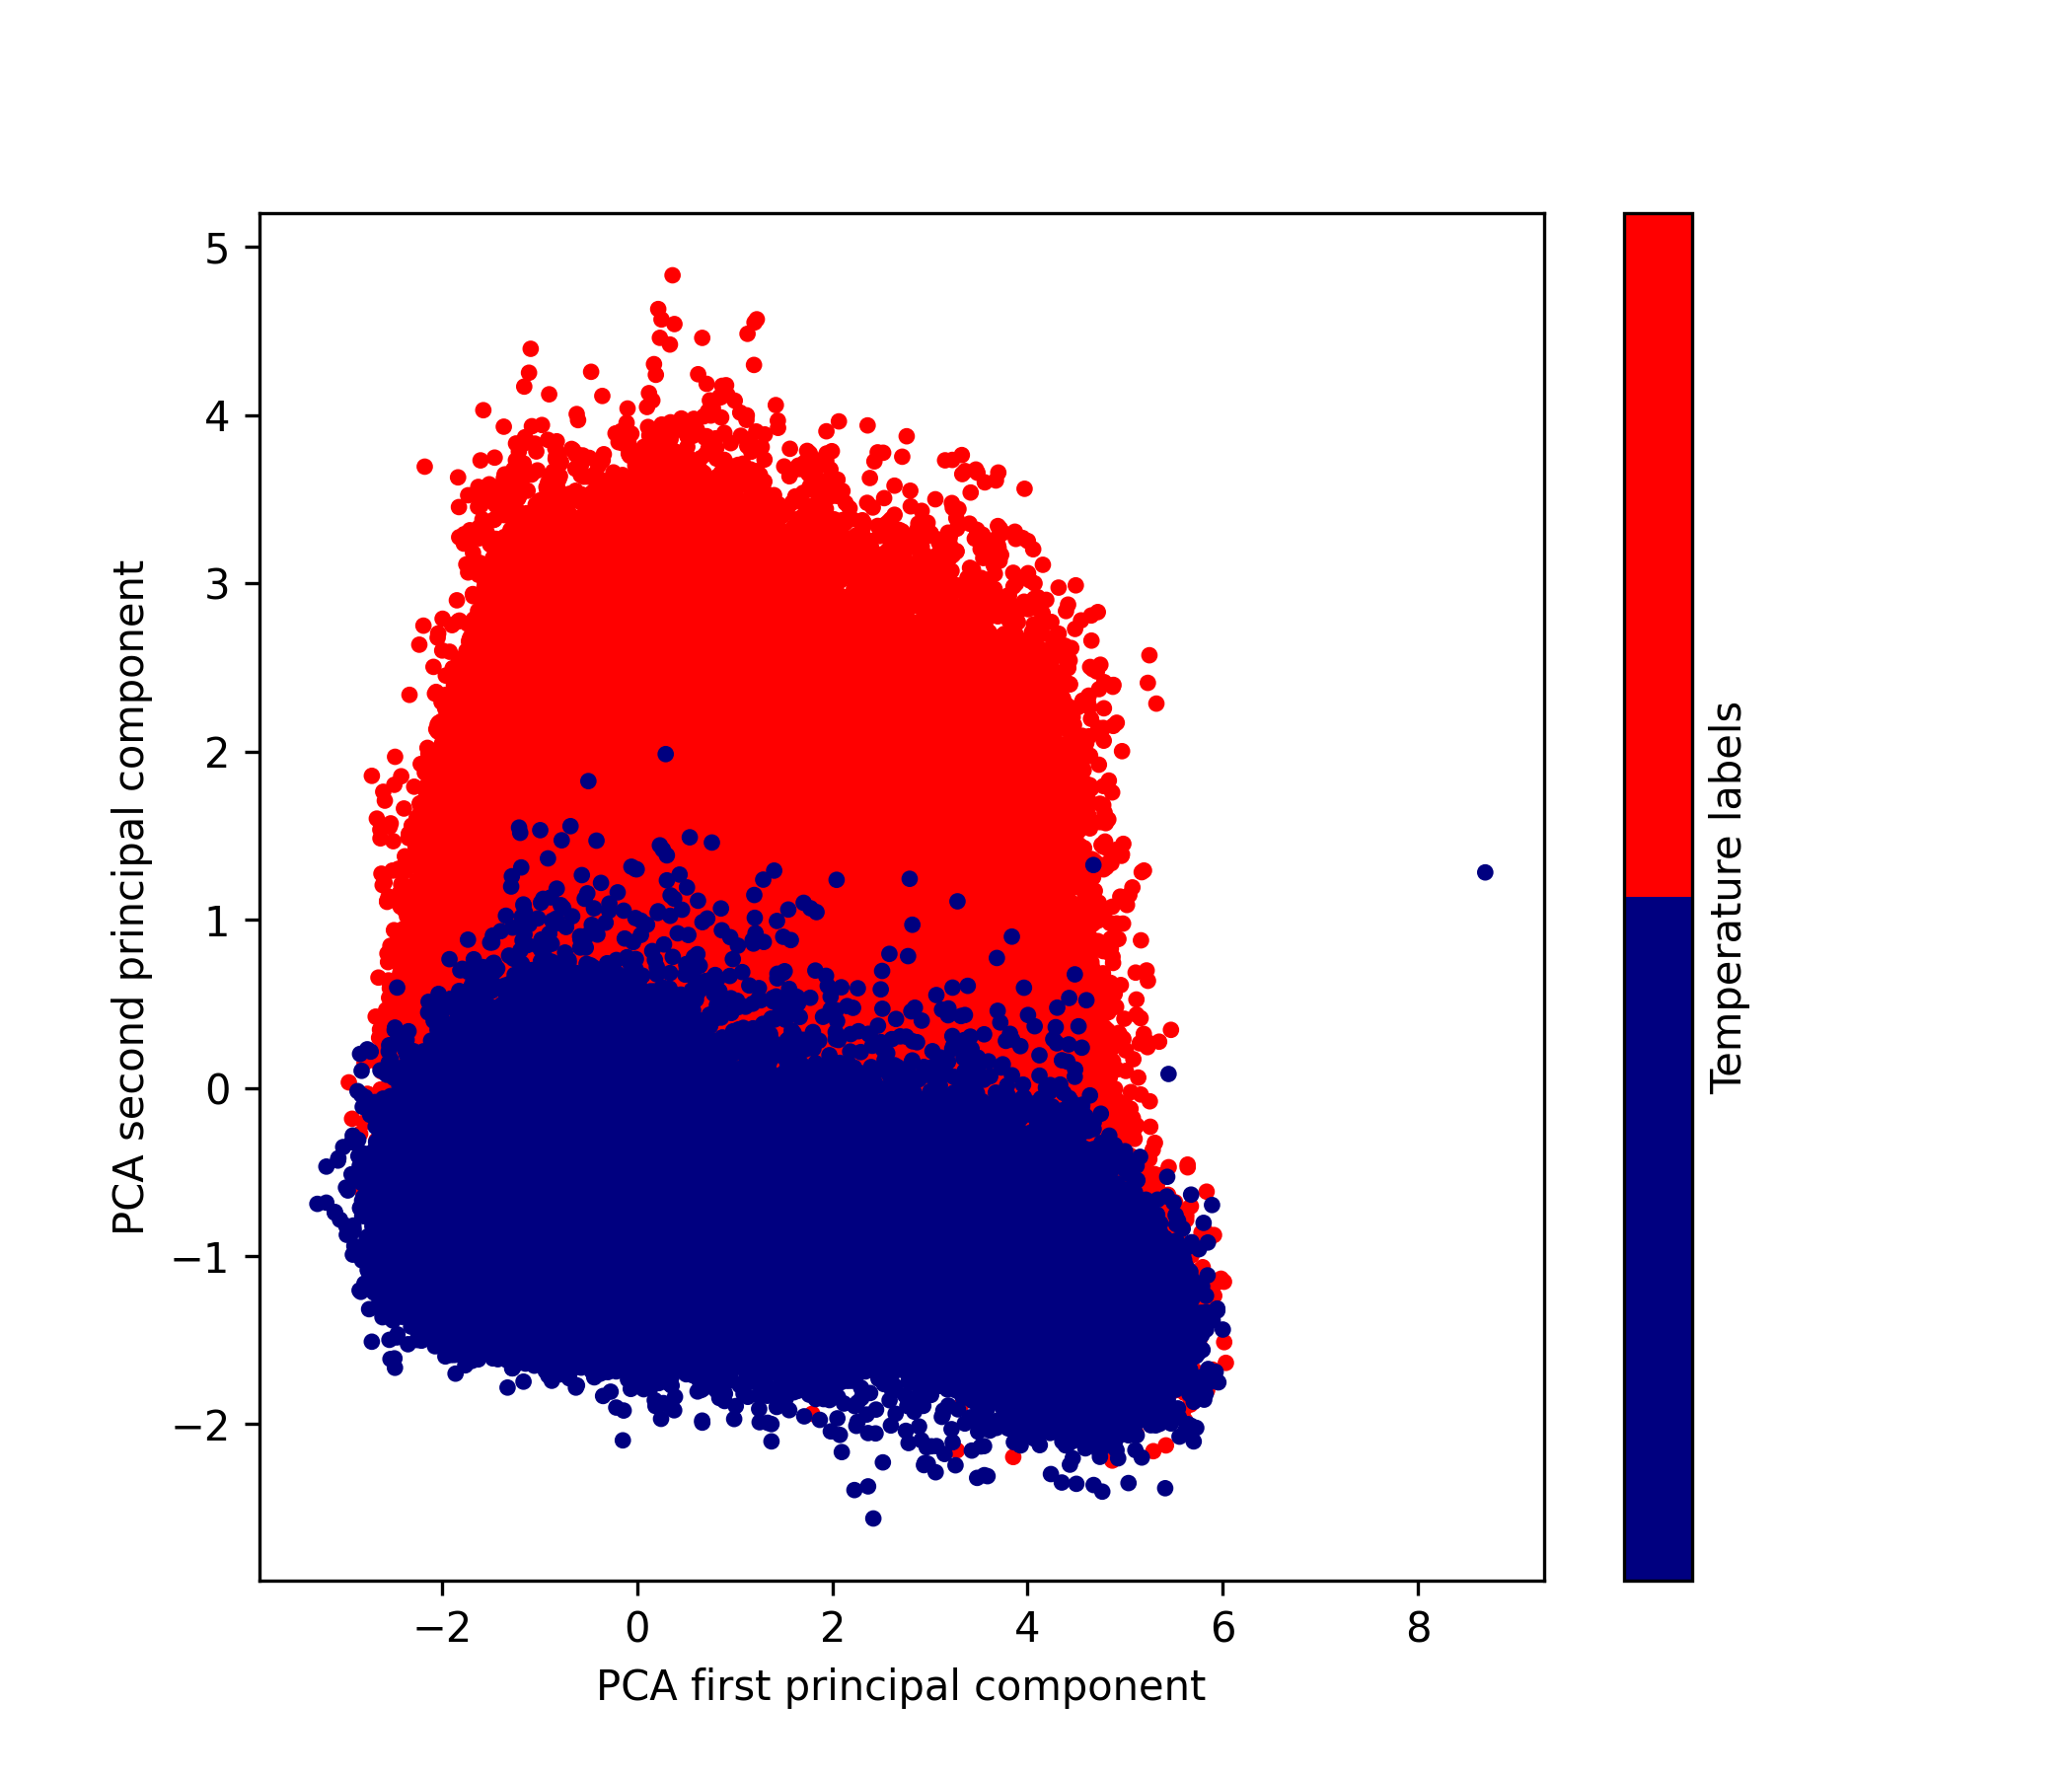
\includegraphics[scale=0.3]{003_train_v2_PCA.png}
		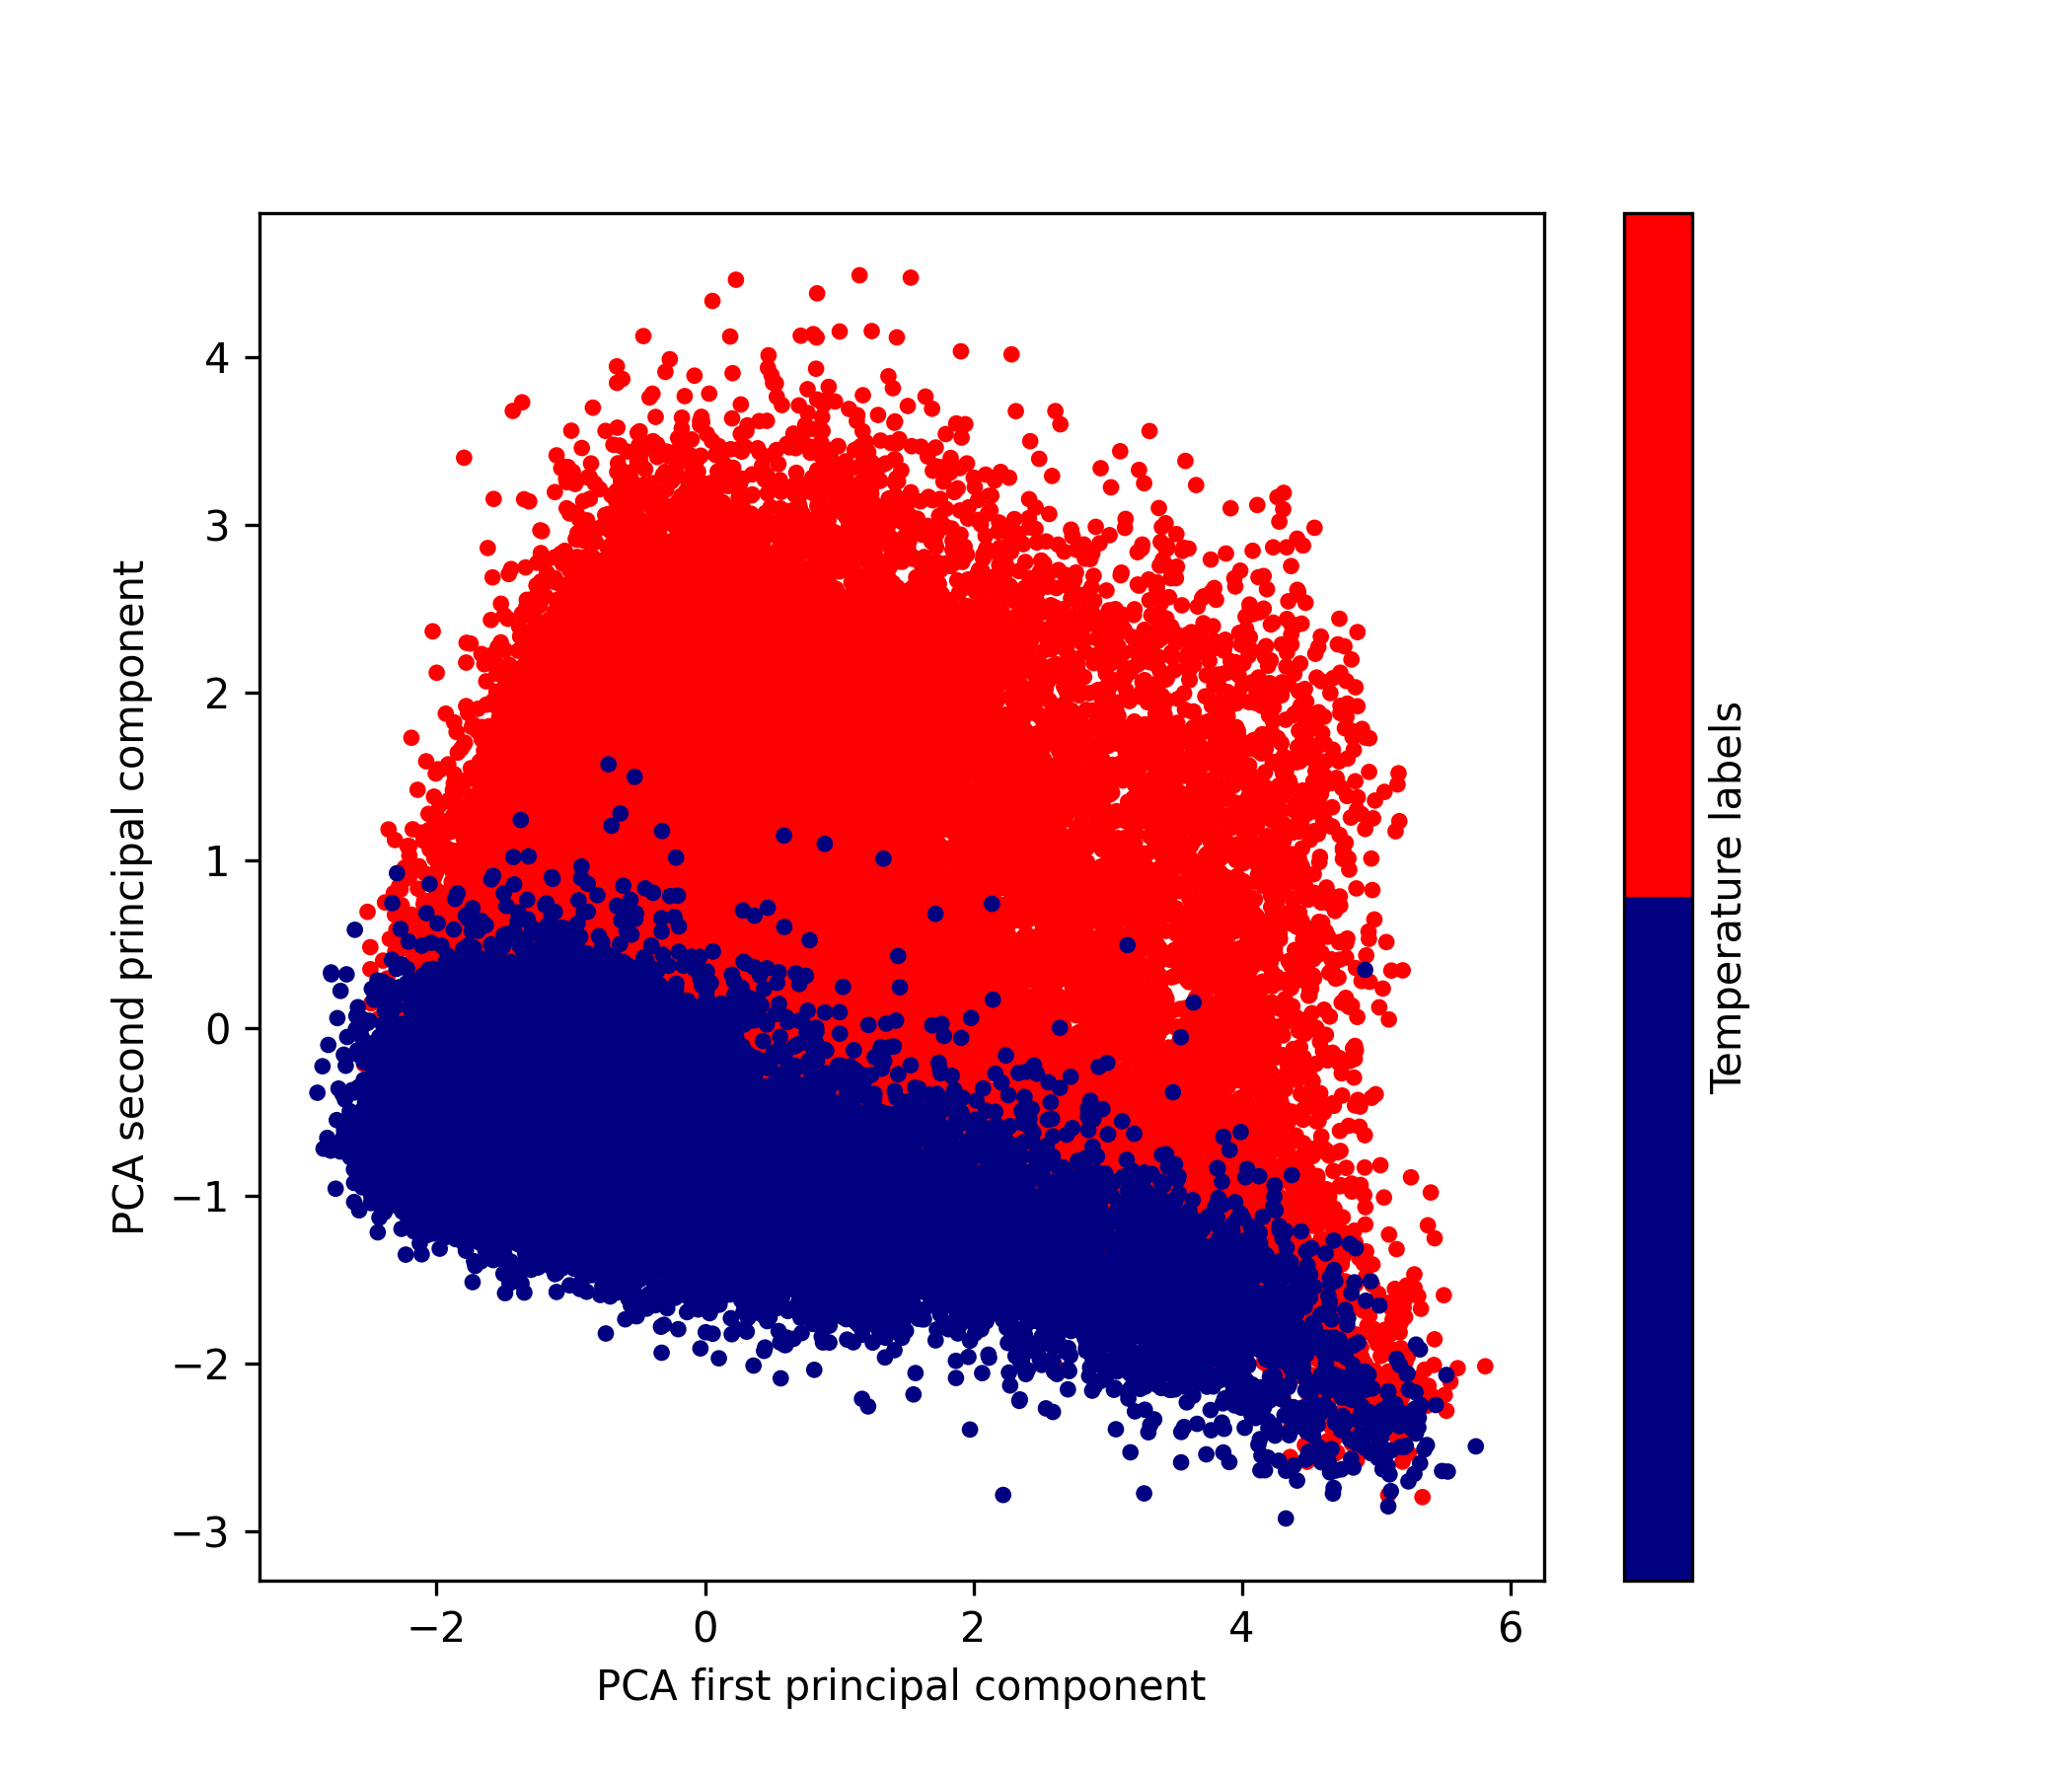
\includegraphics[scale=0.3]{003_validate_v2_PCA.png}

		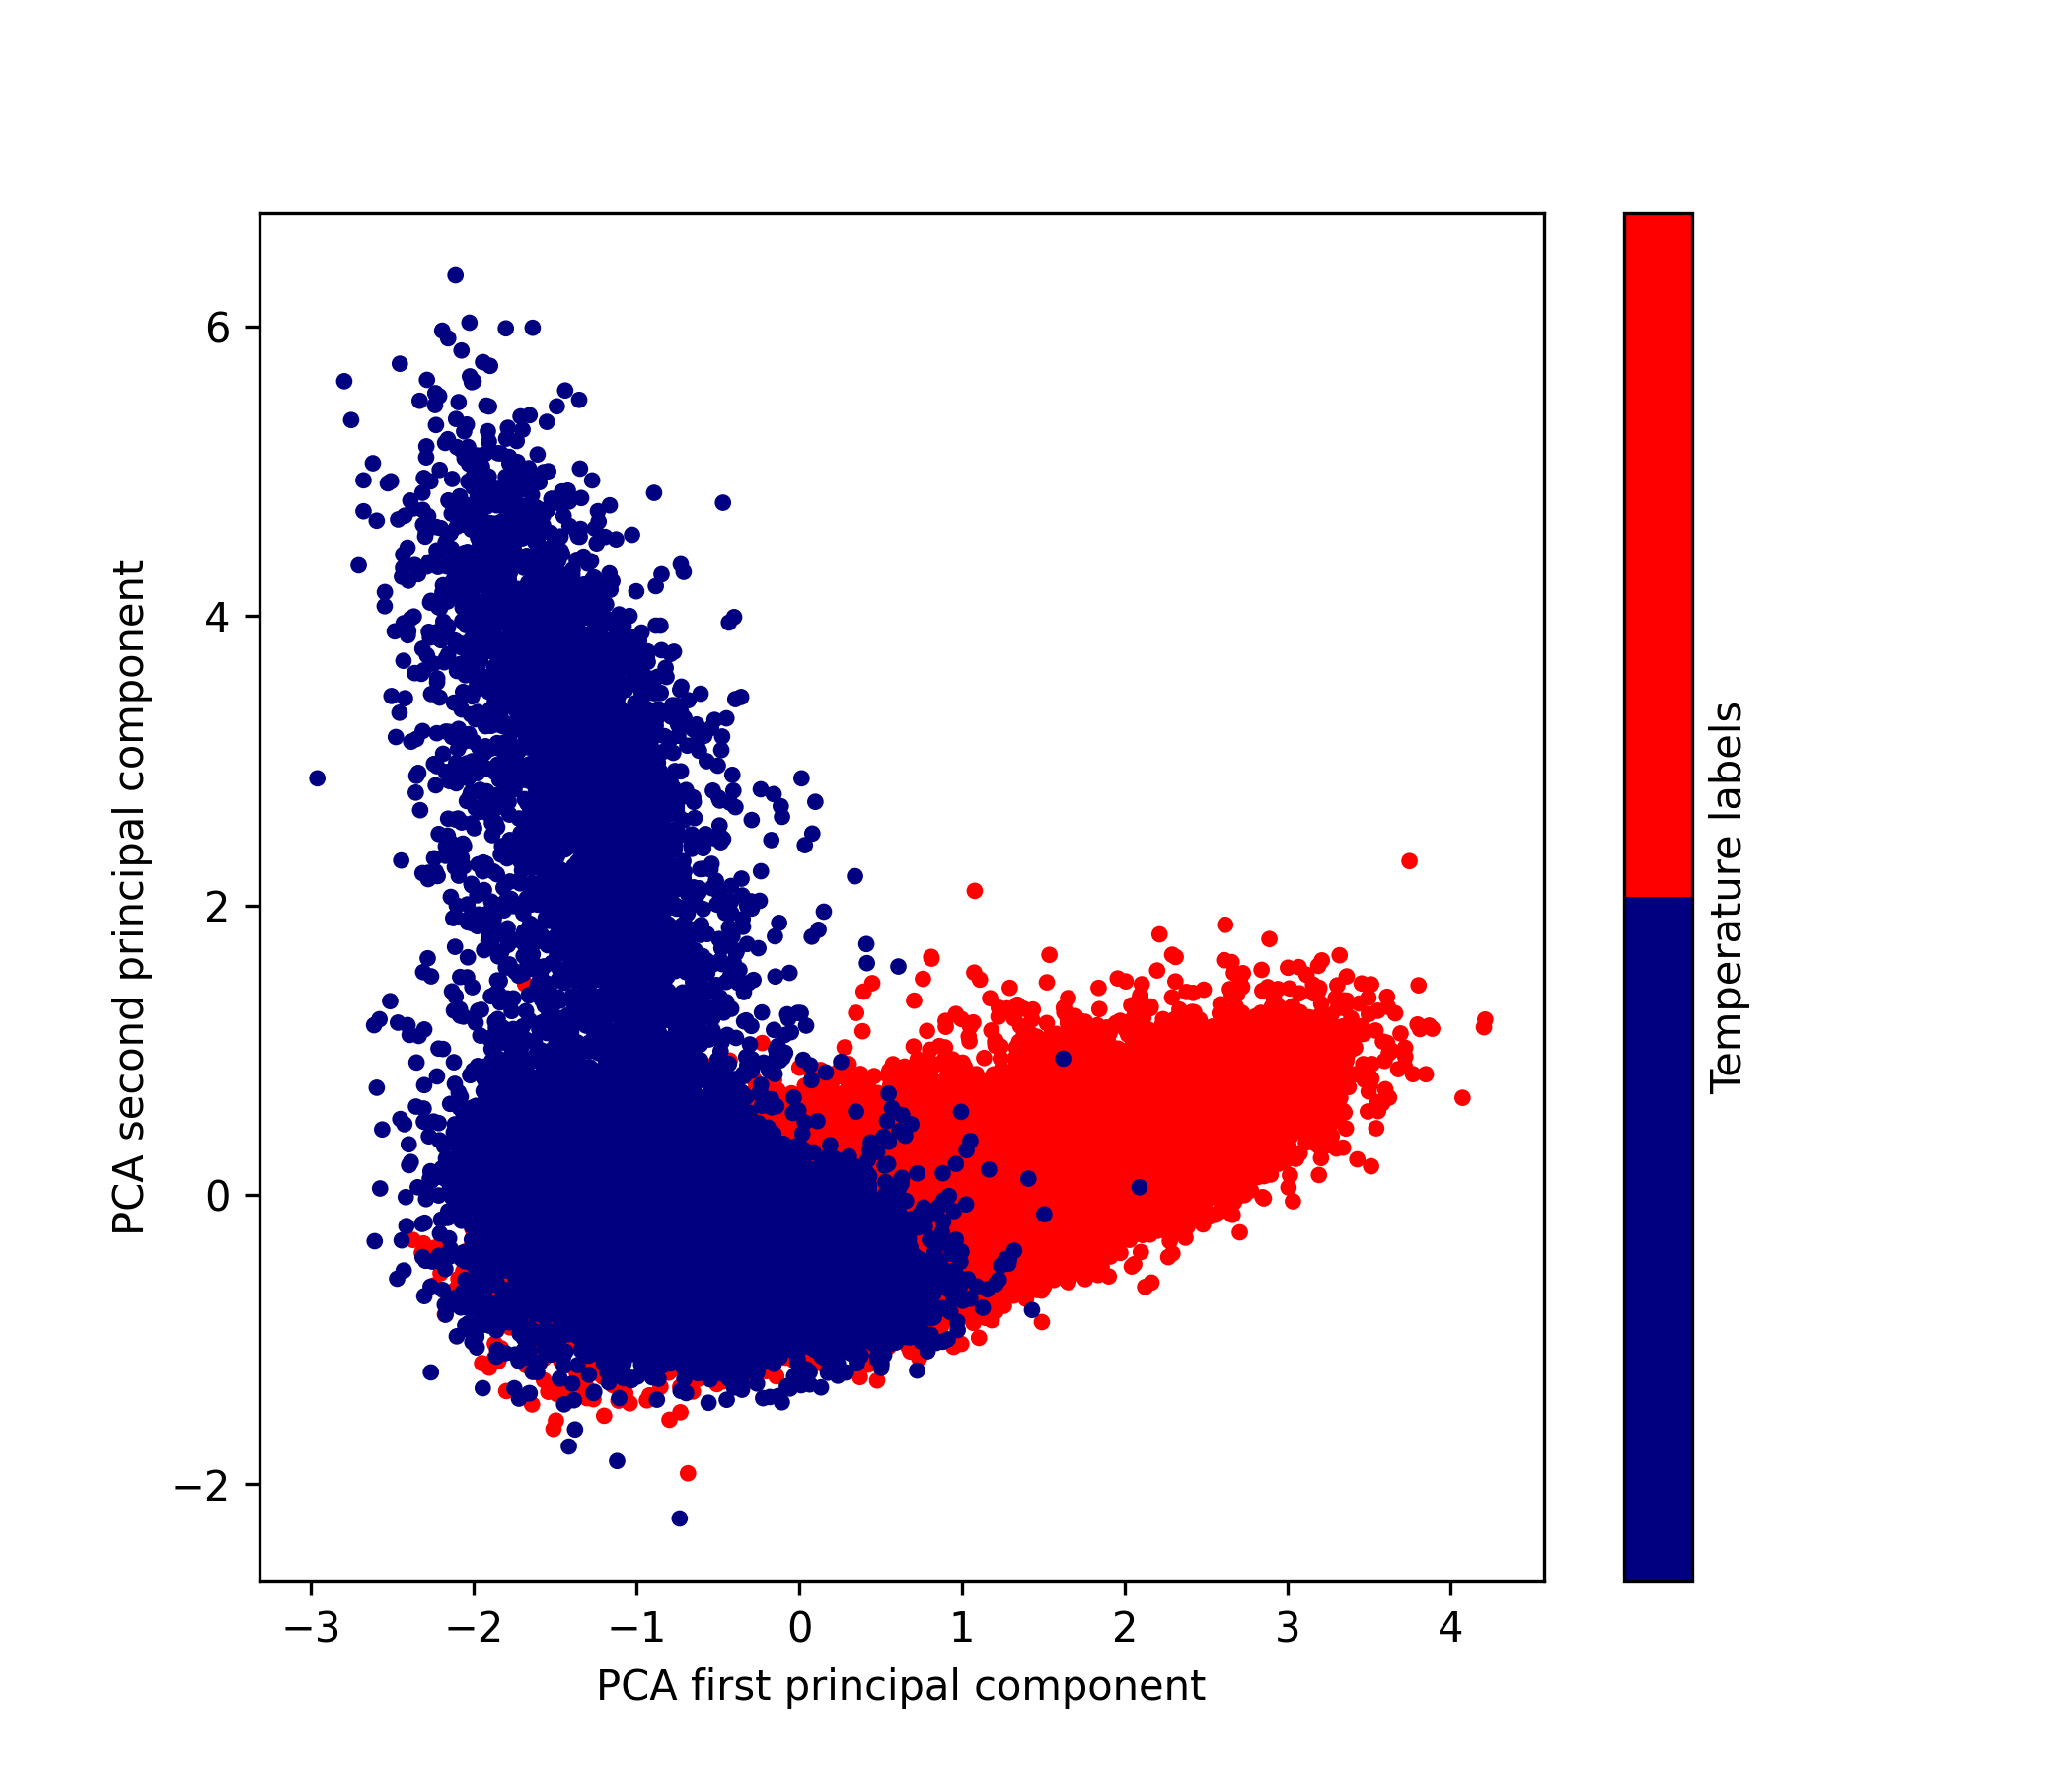
\includegraphics[scale=0.3]{003_test_v2_PCA.png}

		\caption{PCA visualisations of '003' model data sets' embeddings: training set
				in the upper left, validation set in the upper right, and 
				testing set in the lower center}
		\label{figure:ScikitPCAembeddings003}
	\end{figure}
	
	Additionally, \textit{Python} minimum-distortion embedding (\textit{PyMDE}) 
	library (version 0.1.5) was used to visualise data sets of embeddings 
	(Figure \ref{figure:PyMDEPCAembeddings003}), which showed the 3D image
	of data clusters.

	\begin{figure}[h!]
		\centering
		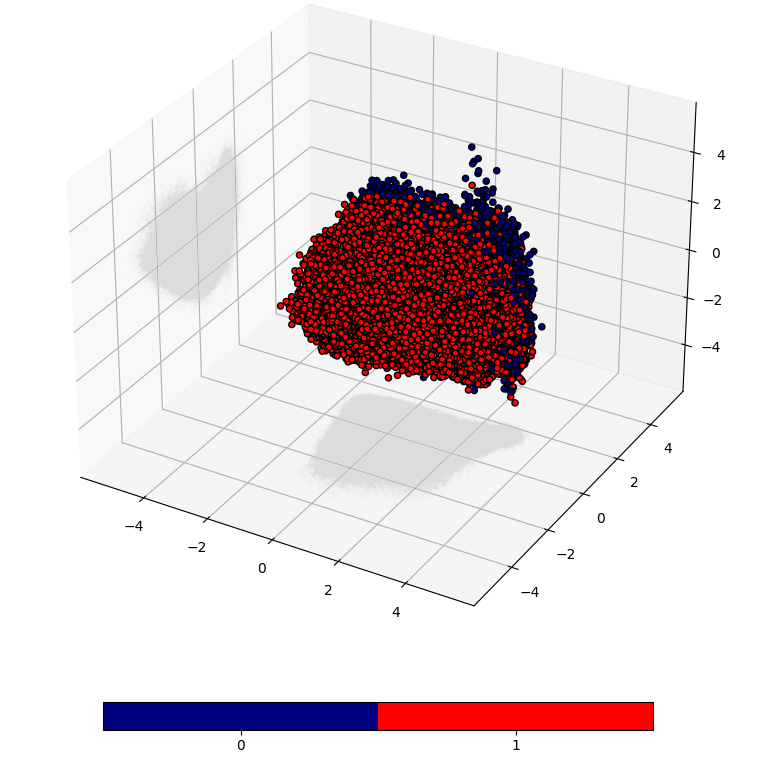
\includegraphics[scale=0.3]{003_train_v2_MDE_PCA.png}
		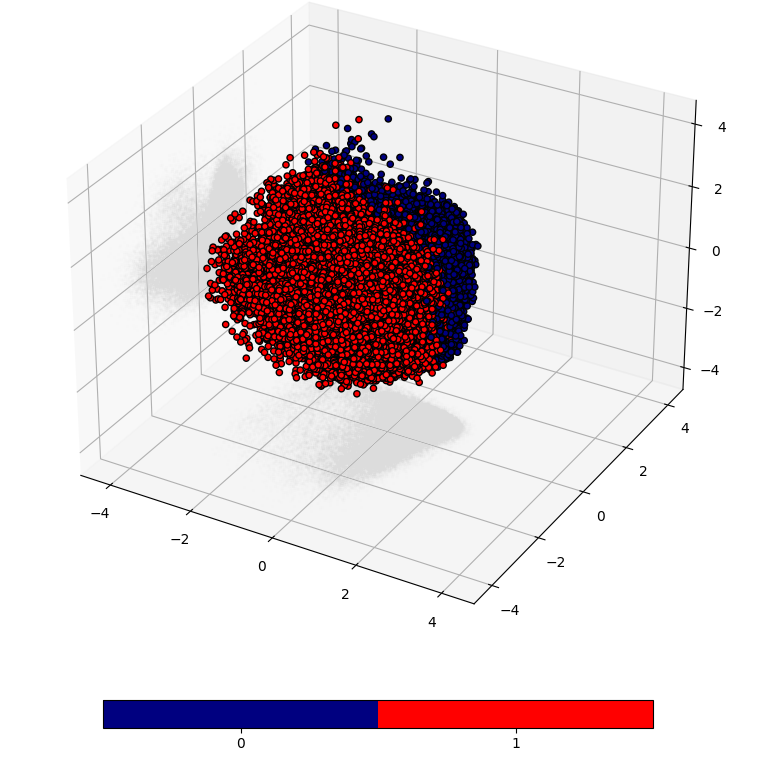
\includegraphics[scale=0.3]{003_validate_v2_MDE_PCA.png}

		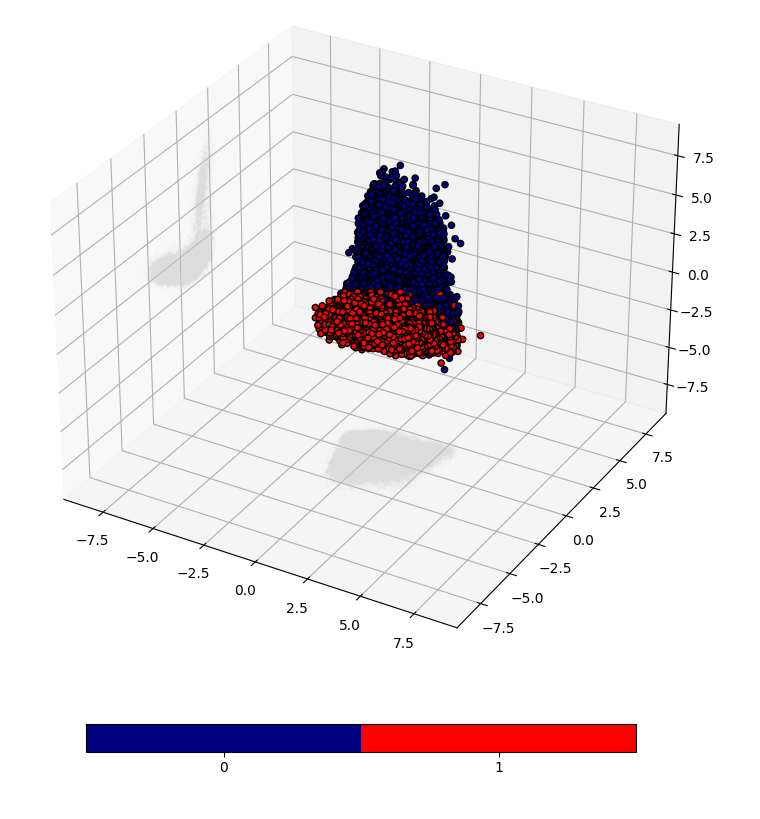
\includegraphics[scale=0.3]{003_test_v2_MDE_PCA.png}

		\caption{\textit{PyMDE} PCA visualisations of '003' model data sets' embeddings: training set
				in the upper left, validation set in the upper right, and 
				testing set in the lower center}
		\label{figure:PyMDEPCAembeddings003}
	\end{figure}

	\newpage

	\subsection{Training and validation of the neural network}

	At first, it was decided to try training the neural network built of
	the most simple architecture - a single layer perceptron (SLP). The input of the 
	layer is 1280-dimensional - it takes the input of protein embeddings - and the 
	output is a binary label that represents the thermostability class. The 
	activation and loss functions were sigmoid and binary cross
	entropy respectively. Adam optimizer with learning rate of 0.0001 was chosen.

	The model was trained and validated in 5 epochs taking mini-batch size of 24
	embeddings. The ROC curves (Figure \ref{figure:SLP003validation4}) did not 
	indicate a significant progress of the training process - the area under 
	the curve was considerably large since the
	first epoch of the training.

	\begin{figure}[h!]
		\centering
		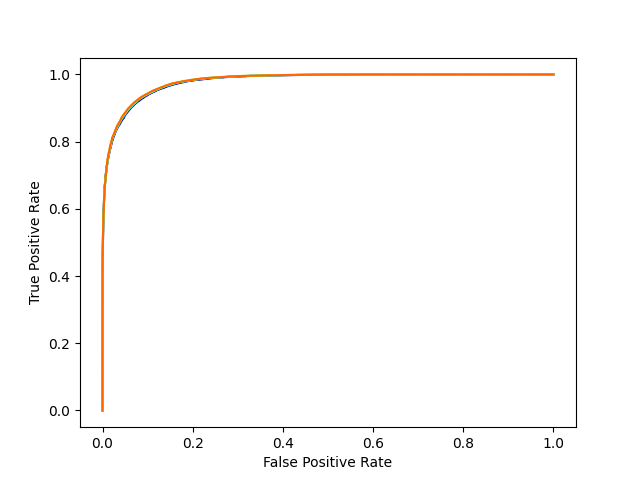
\includegraphics[scale=0.7]{validation_4_2713.png}

		\caption{ ROC curves for each validation epoch - the orange 
		one denotes the curve of the fifth epoch}
		\label{figure:SLP003validation4}
	\end{figure}

	Confusion matrices presented in this work are composed of values in the
	following order reading from left to right: the first row consists of true 
	negative (TN) and false positive (FP) values, the second row consists of 
	false negative (FN) and true positive (TP) values.
	Therefore, the values of the confusion matrix after the fifth training epoch
	showed that most of the mistakes were made by assigning false positive 
	labels to sequences.

	\begin{table}[h!]
		\caption{Confusion matrix after the fifth validation epoch}
		\vspace{0.2cm}
		\centering
		\begin{tabular}{ | c | c c | }
			\hline 
			& 0 & 1 \\
			\hline  
			0 & 32793 & 3636 \\
			1 & 1582 & 30770 \\
			\hline    
		\end{tabular}
		\label{table:SLP003confusionMatrixValidation4}
	\end{table}

	Values in confusion matrix allow to calculate metrics: accuracy, precision,
	and recall. Formulas for calculation of these metrics are given below 
	(Eq. \ref{accuracy}-\ref{recall}).
	The AUC is calculated by integrating the ROC curve. 

	\begin{equation}
		Accuracy = \frac{TP+TN}{TP+FP+TN+FN} 
		\label{accuracy}
	\end{equation}
	\begin{equation}
		Precision = \frac{TP}{TP+FP} 
		\label{precision}
	\end{equation}
	\begin{equation}
		Recall = \frac{TP}{TP+FN} 
		\label{recall}
	\end{equation}

	\begin{table}[h!]
		\caption{Model performance metrics after the fifth validation epoch}
		\vspace{0.2cm}
		\centering
		\begin{tabular}{ | c | c | }
			\hline 
			Accuracy & 0.91989 \\
			Precision & 0.89432 \\
			Recall & 0.9511 \\  
			ROC AUC & 0.92 \\
			\hline 
		\end{tabular}
		\label{table:SLP003metricsValidation4}
	\end{table}

	\section{Results}

	The model was tested with the testing subset of '003' data set that was
	not exposed to the model before the testing stage. 

	The ROC curve (Figure \ref{figure:SLP003testing}) was steep enough to show
	a good performance of the model. The confusion matrix 
	(Table \ref{table:SLP003confusionMatrixTesting}) of the testing stage 
	showed balanced number of mistakes (FP and FN values were approximately 
	equal). Area under testing ROC curve was 0.924, 
	accuracy and precision metrics exceeded those after the fifth training 
	epoch (Table \ref{table:SLP003metricsTesting}). In addition to the metrics
	given for the fifth training epoch, Matthew's correlation coefficient (MCC)
	(\ref{MCC}) was calculated as well.

	\begin{equation}
		\label{MCC}
		MCC = \frac{TP \cdot TN - FP \cdot FN}{\sqrt{(TP+FP)(TP+FN)(TN+FP)(TN+FN)}} 
	\end{equation}

	\begin{figure}[h!]
		\centering
		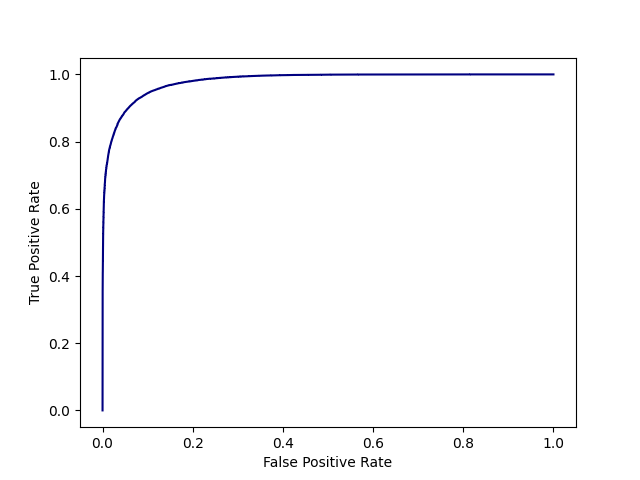
\includegraphics[scale=0.7]{testing_0_3068.png}

		\caption{ ROC curve after the testing stage}
		\label{figure:SLP003testing}
	\end{figure}

	\begin{table}[h!]
		\caption{Confusion matrix in the testing phase}
		\vspace{0.2cm}
		\centering
		\begin{tabular}{ | c | c c | }
			\hline 
			& 0 & 1 \\
			\hline  
			0 & 34933 & 2813 \\
			1 & 2788 & 33122 \\
			\hline    
		\end{tabular}
		\label{table:SLP003confusionMatrixTesting}
	\end{table}

	\begin{table}[h!]
		\caption{Model performance metrics in the testing phase}
		\vspace{0.2cm}
		\centering
		\begin{tabular}{ | c c | }
			\hline 
			Accuracy & 0.924 \\
			Precision & 0.922 \\
			Recall & 0.922 \\
			ROC AUC & 0.924 \\
			MCC & 0.845 \\
			\hline 
		\end{tabular}
		\label{table:SLP003metricsTesting}
	\end{table}

	\newpage

	\section{Conclusions}

	In summary, the objective to develop a tool that predicts the thermostability
	class of the input protein was achieved. Nevertheless, the workflow pointed
	several areas to consider for improvement and future development:

	\begin{itemize}
		\item Overcoming the limitation of sequence length of 1024 amino acids
		\item Experimentation with more sophisticated model architectures
		\item Testing the trained model with per token embeddings and getting 
			  thermostability predictions for each amino acid in the sequence
		\item Picking a different subset of the annotated growth temperatures 
			  data set  
		\item Taking a different kind of embeddings as input
	\end{itemize}
	
	\nocite{*}
	
	\normalsize

\bibliography{references} 
\bibliographystyle{ieeetr}

\end{document}
